\newcommand{\auditoriaid}{A07 -- Resultados y figuras}
% Preambulo comun de las auditorias del informe E1 (revision_e1/)
\documentclass[11pt,a4paper]{article}
\usepackage[utf8]{inputenc}
\usepackage[T1]{fontenc}
\usepackage[spanish,es-noshorthands]{babel}
\usepackage{lmodern}
\usepackage{microtype}
% Sin patrones de guionado en espanol en esta instalacion (ver A10): se
% desactiva el guionado automatico para evitar cortes con reglas del ingles.
\hyphenpenalty=10000
\exhyphenpenalty=10000
\usepackage[a4paper,margin=2.2cm]{geometry}
\usepackage{booktabs,array,longtable}
\usepackage{graphicx,caption,subcaption}
\usepackage{xcolor}
\usepackage{enumitem}
\usepackage{fancyhdr}
\usepackage{amsmath}
\usepackage{tikz}
\usetikzlibrary{arrows.meta,positioning}
\usepackage{natbib}
\usepackage{xurl}
\usepackage[hidelinks]{hyperref}
\urlstyle{tt}
\newcommand{\archivo}[1]{\url{#1}}
\newcolumntype{L}[1]{>{\raggedright\arraybackslash}p{#1}}
\definecolor{alta}{RGB}{180,30,30}
\definecolor{media}{RGB}{200,120,0}
\definecolor{baja}{RGB}{60,110,160}
\definecolor{cajafondo}{RGB}{245,247,250}
\newcommand{\sevA}{\textcolor{alta}{\textbf{Alta}}}
\newcommand{\sevM}{\textcolor{media}{\textbf{Media}}}
\newcommand{\sevB}{\textcolor{baja}{\textbf{Baja}}}
\setlength{\parskip}{0.35em}
\setlength{\emergencystretch}{3em}
\setlength{\parindent}{0pt}
\pagestyle{fancy}
\fancyhf{}
\fancyhead[L]{\small Auditoría del Informe del Entregable~1 -- \auditoriaid}
\fancyhead[R]{\small \thepage}
\renewcommand{\headrulewidth}{0.4pt}
% Entorno de hallazgos: ID | Severidad | Ubicacion | Hallazgo y evidencia | Correccion
\newenvironment{hallazgos}{%
\small
\begin{longtable}{@{}L{1.15cm}L{1.25cm}L{1.9cm}L{6.0cm}L{\dimexpr\textwidth-10.3cm-10.6\tabcolsep\relax}@{}}
\toprule
\textbf{ID} & \textbf{Sev.} & \textbf{Ubicación} & \textbf{Hallazgo y evidencia} & \textbf{Corrección aplicada} \\
\midrule\endfirsthead
\toprule
\textbf{ID} & \textbf{Sev.} & \textbf{Ubicación} & \textbf{Hallazgo y evidencia} & \textbf{Corrección aplicada} \\
\midrule\endhead
\bottomrule\endfoot
}{\end{longtable}}
% Macros compartidas con el informe revisado (las secciones propuestas las usan)
% Macros compartidas entre el informe revisado y las auditorias.
% Cifras verificadas contra los archivos del repositorio (ver A01/A04/A07):
\newcommand{\nUniverso}{102}   % source_id CMIP6 con tos/Omon en ESGF (00b, model_availability_priority.csv)
\newcommand{\nSeed}{41}        % publican los cuatro experimentos (config/models_seed_cmip6.csv)
\newcommand{\nSel}{40}         % completos + QC PASS (models_inventory_final.csv)
\newcommand{\nComb}{160}       % combinaciones modelo-experimento PASS (qc_report.csv)
\newcommand{\nNoEnc}{44}       % config/models_no_encontrado_44.csv
\newcommand{\nParcial}{18}     % 102 - 40 - 44
% Fecha de la portada: fija (no \today), editable en un solo lugar.
\newcommand{\fechaentrega}{28 de septiembre de 2026}
% Estado de codigo que documenta el E1 (antes de los cambios del E2)
\newcommand{\commitEone}{\texttt{8ee6184}}

% En las auditorias el texto propuesto se muestra fuera del informe: las
% referencias cruzadas se imprimen con el nombre de la seccion destino.
\makeatletter
\def\etq#1#2{\expandafter\def\csname etq@#1\endcsname{#2}}
\etq{sec:resumen}{Resumen}
\etq{sec:alcance}{Alcance}
\etq{sec:marco}{Revisión científica}
\etq{sec:antecedentes}{Antecedentes}
\etq{sec:referencias}{Literatura sobre TOE}
\etq{tab:referencias}{bibliografía TOE}
\etq{sec:similitudes}{Niño~3.4 frente a Niño~1+2}
\etq{sec:toe_metodos}{Elección de los métodos de TOE}
\etq{tab:metodos_toe}{métodos TOE}
\etq{eq:szabo_signal}{ecuación señal M1}
\etq{eq:szabo_V}{ecuación V(t)}
\etq{eq:szabo_T}{ecuación T(t)}
\etq{eq:szabo_toe}{ecuación TOE M1}
\etq{eq:tod}{ecuación ToD}
\etq{sec:datos}{Datos}
\etq{fig:cmip6_contribution}{contribución institucional}
\etq{sec:tabla_modelos}{Modelos seleccionados}
\etq{tab:modelos}{modelos}
\etq{sec:desviacion}{Selección de modelos}
\etq{sec:dominios_periodos}{Dominios y periodos}
\etq{fig:region_nino}{regiones Niño}
\etq{sec:arquitectura}{Arquitectura del pipeline}
\etq{fig:flujograma}{Flujograma}
\etq{sec:scripts}{Descripción de los pasos}
\etq{sec:paso00b}{Paso 00b}
\etq{sec:paso01}{Paso 01}
\etq{sec:paso02}{Paso 02}
\etq{sec:paso04}{Paso 04}
\etq{sec:paso05}{Paso 05}
\etq{sec:paso06}{Paso 06}
\etq{sec:paso07}{Paso 07}
\etq{sec:reporte}{Reporte de estado}
\etq{sec:resultados}{Resultados}
\etq{fig:qc}{matriz de estado}
\etq{tab:cuentas}{conteo de modelos}
\etq{fig:mapas2d}{mapas 2D}
\etq{fig:series}{series}
\etq{fig:boxplot}{boxplots}
\etq{sec:roadmap}{Próximos pasos}
\etq{tab:roadmap}{próximos pasos}
\etq{sec:conclusiones}{Conclusiones}
\etq{sec:recomendaciones}{Recomendaciones}
\makeatother

\makeatletter
\AtBeginDocument{\renewcommand{\ref}[1]{\@ifundefined{etq@#1}{\textit{[#1]}}{\textit{\csname etq@#1\endcsname}}}}
\makeatother
% Texto propuesto: secciones degradadas un nivel y en caja
\newenvironment{propuesto}{%
  \par\medskip\noindent\textcolor{baja}{\rule{\textwidth}{0.8pt}}\par
  \noindent{\small\textbf{Inicio del texto propuesto para el informe revisado}}\par\medskip
  \begingroup
  \let\section\subsection\let\subsection\subsubsection\let\subsubsection\paragraph
}{%
  \endgroup
  \par\noindent{\small\textbf{Fin del texto propuesto}}\par
  \noindent\textcolor{baja}{\rule{\textwidth}{0.8pt}}\par\medskip}
% Recuadro de actualizacion posterior (decisiones del autor)
\newcommand{\actualizacion}[1]{\par\medskip\noindent\fcolorbox{media}{media!8}{\parbox{\dimexpr\linewidth-2\fboxsep-2\fboxrule\relax}{\small\textbf{Actualización del 29-09-2026 (decisiones del autor).} #1}}\par\medskip}

\graphicspath{{../}}
\begin{document}

\begin{center}
{\Large\bfseries Auditoría A07: Resultados y figuras}\\[0.4em]
{\normalsize Informe del Entregable~1, Sección~7 (\texttt{informe\_e1\_smnv3.tex}, commit \texttt{330fd2e})}\\[0.2em]
{\small Revisión: \fechaentrega}
\end{center}

\section{Objeto}

Se audita la Sección~7: cifras de resultado, matriz de estado, mapas 2D, series y \emph{boxplots}. Las cifras se recalcularon desde los CSV. Cada figura se regeneró desde el código del E1 y se comparó con la que hoy incluye el PDF. Las figuras que usa el informe son enlaces simbólicos a \archivo{figures/} (ver A04-5), así que el PDF muestra lo que haya en esa carpeta al momento de compilar.

\actualizacion{Los mapas 2D muestran ahora toda la ventana vigente (0°--360°, 30°S--30°N). Las demás figuras (matriz de estado, series y \emph{boxplots}) dependen de las cajas y no cambian.}

\section{Verificación de cifras}

\begin{center}\small
\begin{tabular}{@{}lrl@{}}
\toprule
Afirmación & Valor & Estado \\
\midrule
Modelos seleccionados / universo & 40 / 102 & Correcto \\
Combinaciones PASS & 160 / 160 & Correcto \\
No encontrados en ninguna fuente & 44 & Correcto \\
``Un subconjunto adicional'' con descarga parcial & 18 & Sin cifra en el informe (A07-6) \\
``Tres modelos de grilla nativa más gruesa'' & 9 modelos a 250\,km & Incorrecto (A07-3) \\
\bottomrule
\end{tabular}
\end{center}

\section{Defectos encontrados en las figuras}

\textbf{\emph{Boxplots} desactualizados.} La figura del PDF muestra 31 modelos, no los 40 que dice el pie. Faltan ACCESS-CM2, CAS-ESM2-0, CMCC-CM2-SR5, EC-Earth3, EC-Earth3-Veg, GISS-E2-1-G, GISS-E2-1-H, KACE-1-0-G y UKESM1-0-LL. El script grafica todos los modelos \texttt{selected=True}, pero es idempotente: al existir el PNG, no lo regenera salvo que el usuario responda ``sí'' en los 15\,s de la pregunta. Si la última regeneración ocurrió con 31 modelos seleccionados, la figura quedó congelada. Regenerada con el inventario actual, muestra los 40.

\textbf{Periodo común mal calculado.} El título de la figura dice ``116 años comunes: 1900--2015'', pero ningún \texttt{historical} pasa de 2014. La causa está en \texttt{plot\_common.box\_mean}, que asigna a cada mes el año decimal $\text{año}+(\text{mes}-0{,}5)/12$, y en los dos scripts que lo redondean con \texttt{np.round}: de julio a diciembre cuentan como el año siguiente. En ERSSTv5, que continúa después de 2014, entran así los meses de enero a junio de 2015. El mismo redondeo afecta a las medianas de las series. El efecto numérico es pequeño (seis meses sobre 1380), pero el periodo reportado es falso. En la copia local se corrigió con \texttt{np.floor}: 115 años, 1900--2014.

\textbf{Mapas 2D y regiones.} Muestran la ventana del E2 (ver A04-5). El pie de los mapas dice ``temperatura superficial del mar media del periodo histórico común (mes de muestra 1950-12)'', lo que es contradictorio: el script grafica un único mes, diciembre de 1950.

\textbf{Idioma.} Los ejes de las figuras mezclan inglés (\emph{Latitude}, \emph{Year}, \emph{ERSSTv5 median}, \emph{Pass}) con español sin tildes (\emph{periodo historico}, \emph{anios}, \emph{degC}). En la copia local se uniformaron al español.

Todas las correcciones de figuras se hicieron \emph{solo} en \archivo{revision_e1/trabajo/e1_snapshot/}; el código del repositorio no se modificó. La recomendación de llevarlas al repositorio está en A10.

\section{Resultado nuevo que el informe no reportaba}

Con las figuras corregidas se cuantificó la diferencia entre las medianas de cada modelo y la de ERSSTv5 (1900--2014):

\begin{center}\small
\begin{tabular}{@{}lrrrrr@{}}
\toprule
Caja & Mediana ERSSTv5 & Sesgo mediano & Rango & Cálidos $>+0{,}5$\,°C & Fríos $<-0{,}5$\,°C \\
\midrule
Niño~3.4 & 26{,}78\,°C & $-0{,}24$\,°C & $-1{,}95$ a $+1{,}12$ & 4 & 16 \\
Niño~1+2 & 22{,}54\,°C & $+2{,}21$\,°C & $+0{,}18$ a $+4{,}53$ & 38 & 0 \\
\bottomrule
\end{tabular}
\end{center}

Hay un sesgo cálido casi universal en Niño~1+2. Es coherente con la literatura revisada (A03) y relevante para el Entregable~2. Se incorpora al texto como observación preliminar, sin anticipar la evaluación formal.

\section{Hallazgos}

\begin{hallazgos}
A07-1 & \sevA & Fig.~boxplot & El PDF muestra 31 modelos y el pie dice 40. & Figura regenerada con los 40. \\
A07-2 & \sevA & Fig.~boxplot & Periodo ``1900--2015'' por redondeo del año decimal. & Corregido en la copia local (1900--2014); se recomienda corregir los tres scripts afectados en el repositorio (A10). \\
A07-3 & \sevA & 7, párr.~3 & ``los tres modelos de grilla nativa más gruesa entre los 40 seleccionados'': hay 9 modelos con 250\,km (Cuadro de modelos). & ``tres de los nueve modelos de resolución nominal más gruesa''. \\
A07-4 & \sevA & Mapas 2D y regiones & Muestran una ventana distinta de la que describía el texto. & \textit{Actualización 29-09}: regenerados para toda la ventana vigente (0°--360°, 30°S--30°N), y el texto se ajustó a ella. \\
A07-5 & \sevM & Pie de mapas & ``media del periodo \ldots\ (mes de muestra 1950-12)'': es un único mes. & ``un mes de muestra (diciembre de 1950)''. \\
A07-6 & \sevM & 7, párr.~1 & ``un subconjunto adicional quedó con descarga parcial'' sin cifra; el cierre $102=40+44+?$ queda incompleto. & Cuadro nuevo con el paso de 102 a 40 (incluye 49 y 41; ver A04-4). \\
A07-7 & \sevM & 7 & No se informa que el QC final no tuvo rechazos, dato que el lector necesita para interpretar la matriz. & Una frase. \\
A07-8 & \sevM & 7, cierre & No hay lectura alguna de los \emph{boxplots}; el sesgo cálido de Niño~1+2 es el hallazgo más visible. & Párrafo cuantitativo, presentado como preliminar. \\
A07-9 & \sevB & Pie de series & Menciona la ruta \archivo{figures/<M00X>_serie_..._Nino1+2.png}, un detalle de uso. & Se indica que las series de Niño~1+2 se entregan junto con las demás figuras. \\
A07-10 & \sevB & 7 & ``(Figuras~\ref{fig:boxplot})'' en plural para una sola figura; ``línea roja punteada'' cuando el código usa línea discontinua (\texttt{--}). & Corregido. \\
A07-11 & \sevB & Figuras & Etiquetas en tres idiomas o variantes. & Uniformadas al español. \\
\end{hallazgos}

\section{Figura regenerada (\emph{boxplot} de Niño~1+2)}

\begin{center}
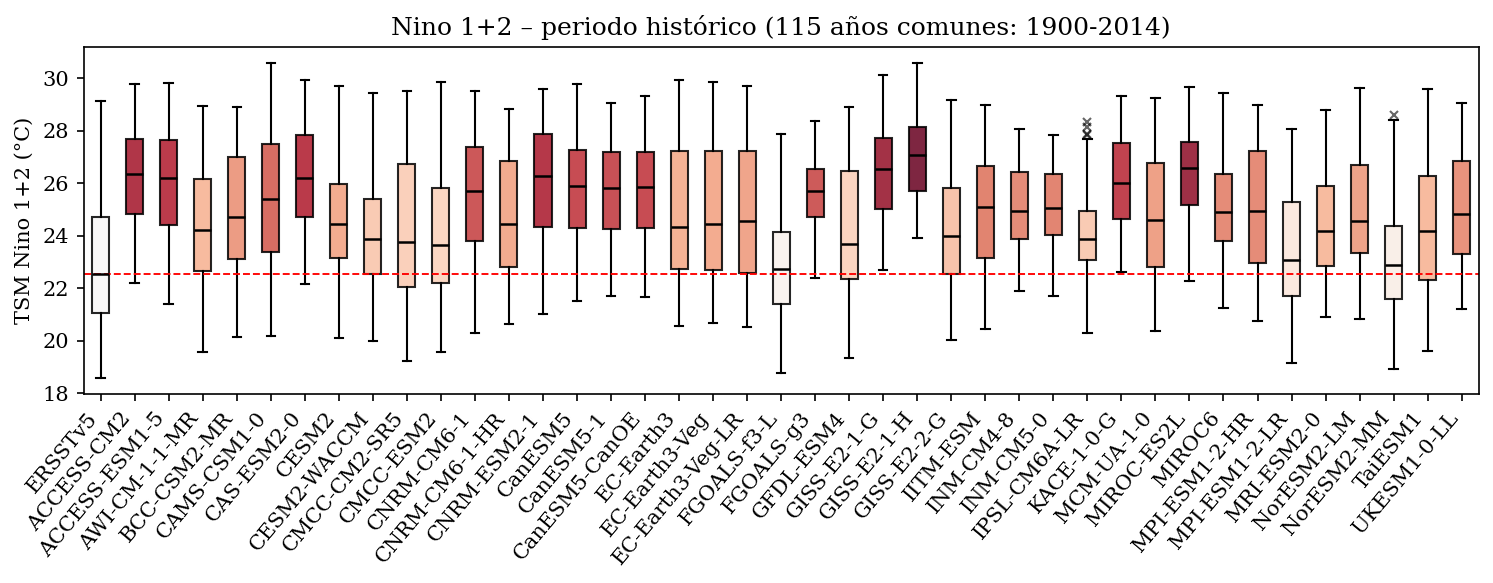
\includegraphics[width=\textwidth]{figuras/boxplot_Nino1+2.png}
\end{center}

\section{Extensión}

Original: 952 palabras. Propuesto: 904 
palabras.

\section{Texto propuesto}

\begin{propuesto}
% ============================================================
\section{Resultados del Entregable~1}
\label{sec:resultados}
% ============================================================

Del universo de 102 modelos CMIP6 que publican \texttt{tos}/\texttt{Omon} en ESGF, 40 completaron los cuatro experimentos requeridos y aprobaron el control de calidad final: 160 combinaciones modelo-experimento, todas con estado \texttt{PASS}. El Cuadro~\ref{tab:cuentas} resume cómo se llega a esa cifra.

\begin{table}[htbp]
\centering
\caption{Del universo de modelos candidatos al conjunto seleccionado.}
\label{tab:cuentas}
\small
\begin{tabular}{@{}L{9.6cm}rL{\dimexpr\textwidth-9.6cm-1.2cm-6\tabcolsep\relax}@{}}
\toprule
\textbf{Conjunto} & \textbf{Modelos} & \textbf{Fuente} \\
\midrule
Publican \texttt{tos}/\texttt{Omon} en ESGF (universo) & 102 & Paso~00b \\
Publican \texttt{historical}, \texttt{ssp245} y \texttt{ssp585} & 49 & Paso~00b \\
Publican además \texttt{ssp370} (lista de descarga) & 41 & Paso~00b \\
Completos y aprobados en el control de calidad (seleccionados) & 40 & Pasos~06--07 \\
\midrule
Excluidos: algún experimento no disponible en ninguna fuente consultada & 44 & Pasos~00b--02 \\
Excluidos: disponibilidad o descarga incompleta & 18 & Pasos~00b--02 \\
\bottomrule
\end{tabular}
\end{table}

La Figura~\ref{fig:qc} muestra el estado de cada modelo y experimento para el universo completo. Cada celda toma uno de seis estados: aprobado (el archivo se descargó y pasó el control de calidad); rechazado (se descargó pero no lo pasó); descarga pendiente (existe un enlace de descarga activo pero el archivo aún no se descargó o procesó); sin enlace (el Paso~00b encontró el experimento, pero el Paso~01 no encontró ningún enlace activo); solo \texttt{hist-1950} (el modelo publica la variante HighResMIP 1950--2014 en lugar de \texttt{historical}; estos modelos no corren los SSP estándar y nunca reúnen los cuatro experimentos); y no disponible (el experimento no existe en ningún nodo consultado). En la corrida final no quedó ningún archivo rechazado.

\begin{figure}[htbp]
\centering
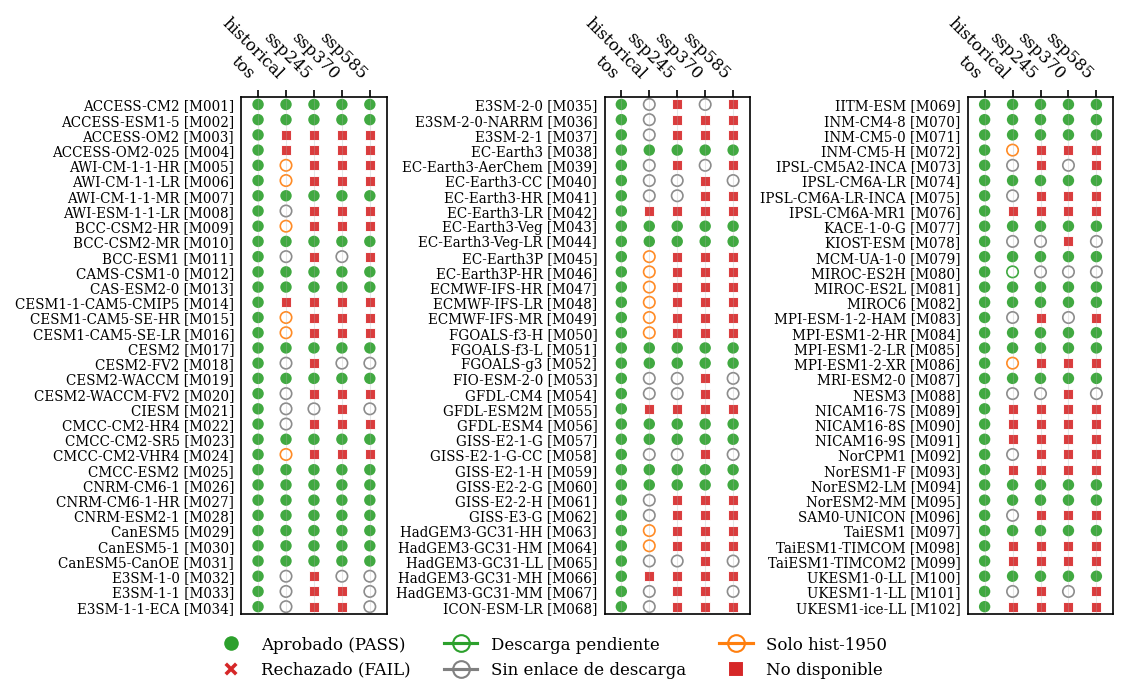
\includegraphics[width=\textwidth]{figuras/sst_QD_vf.png}
\caption[Disponibilidad y control de calidad de \texttt{tos}/\texttt{Omon} para los 102 modelos candidatos.]{Estado por modelo (nombre y código \texttt{M001}--\texttt{M102}) y por columna (\texttt{tos}, \texttt{historical}, \texttt{ssp245}, \texttt{ssp370}, \texttt{ssp585}) para los 102 modelos candidatos. Los 40 modelos seleccionados son los que tienen las cinco columnas aprobadas.}
\label{fig:qc}
\end{figure}

Como verificación exploratoria de la homogeneización, se compara ERSSTv5 con tres de los nueve modelos seleccionados de resolución nominal más gruesa, 250\,km: ACCESS-CM2, ACCESS-ESM1-5 y GISS-E2-1-G (Cuadro~\ref{tab:modelos}). Son los casos en que el regrillado a la grilla de ERSSTv5 es más exigente. Estas figuras, junto con la matriz de estado y las comparaciones por caja, las genera automáticamente \texttt{run.sh} al final de cada corrida (\archivo{scripts/plot_*.py}).

\begin{figure}[htbp]
\centering
\begin{subfigure}[t]{0.75\textwidth}
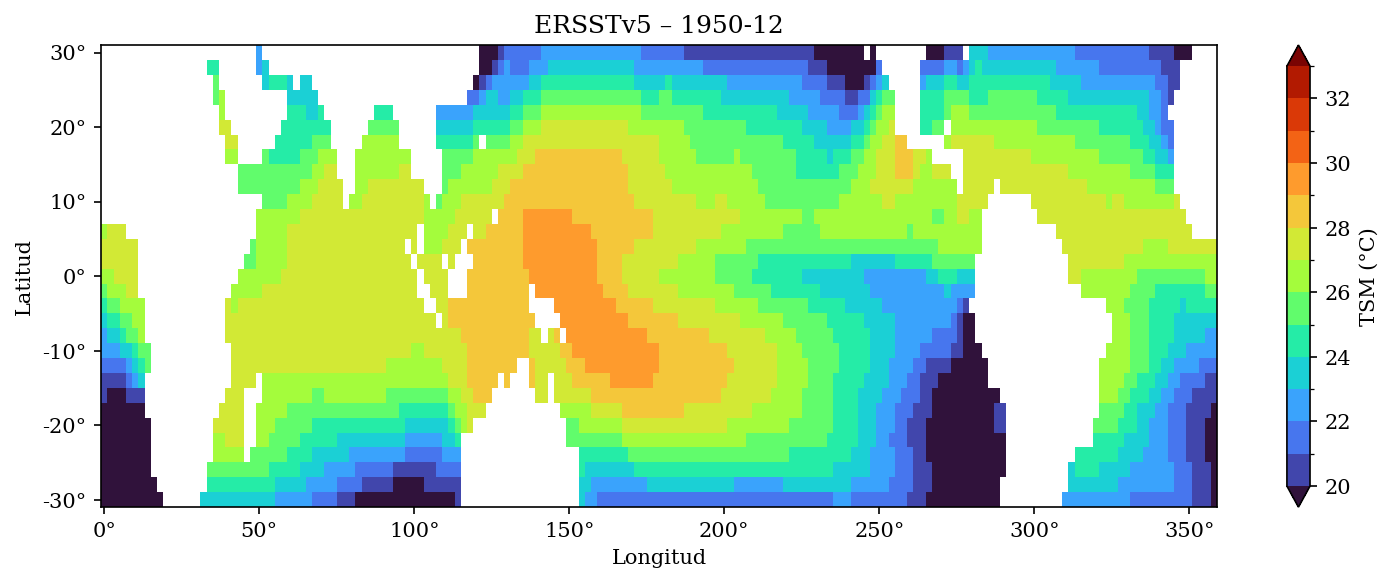
\includegraphics[width=\textwidth]{figuras/sst_2d_ERSSTv5.png}
\end{subfigure}
\begin{subfigure}[t]{0.75\textwidth}
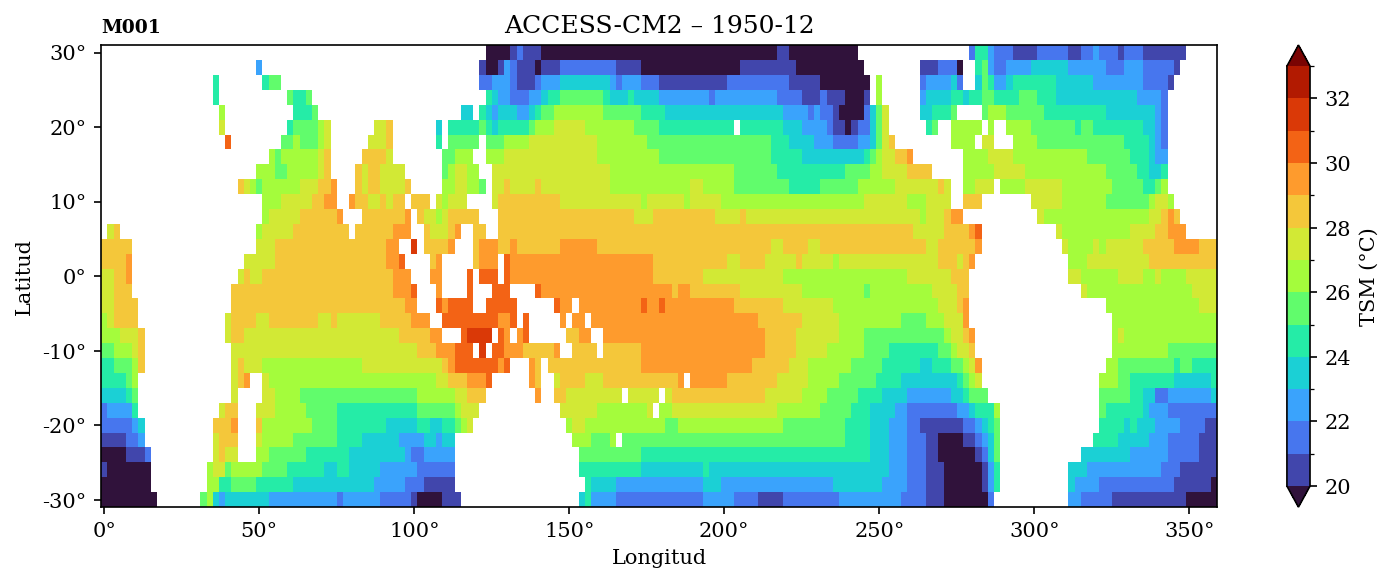
\includegraphics[width=\textwidth]{figuras/M001_sst_2d_ACCESS-CM2.png}
\end{subfigure}
\begin{subfigure}[t]{0.75\textwidth}
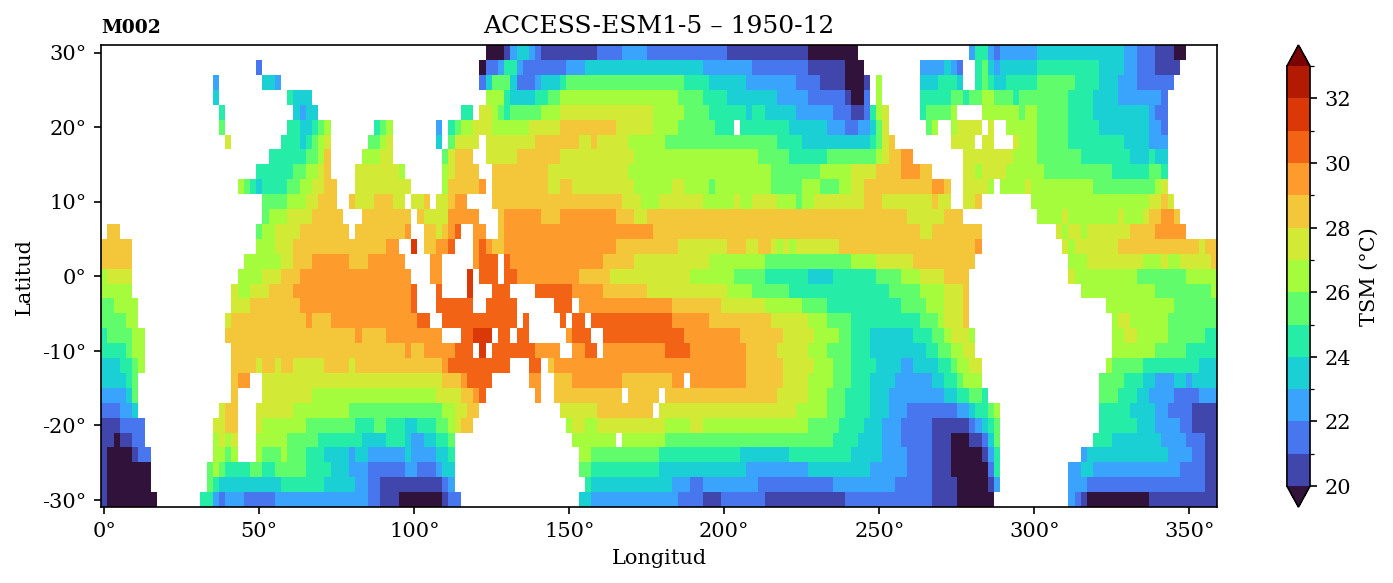
\includegraphics[width=\textwidth]{figuras/M002_sst_2d_ACCESS-ESM1-5.png}
\end{subfigure}
\begin{subfigure}[t]{0.75\textwidth}
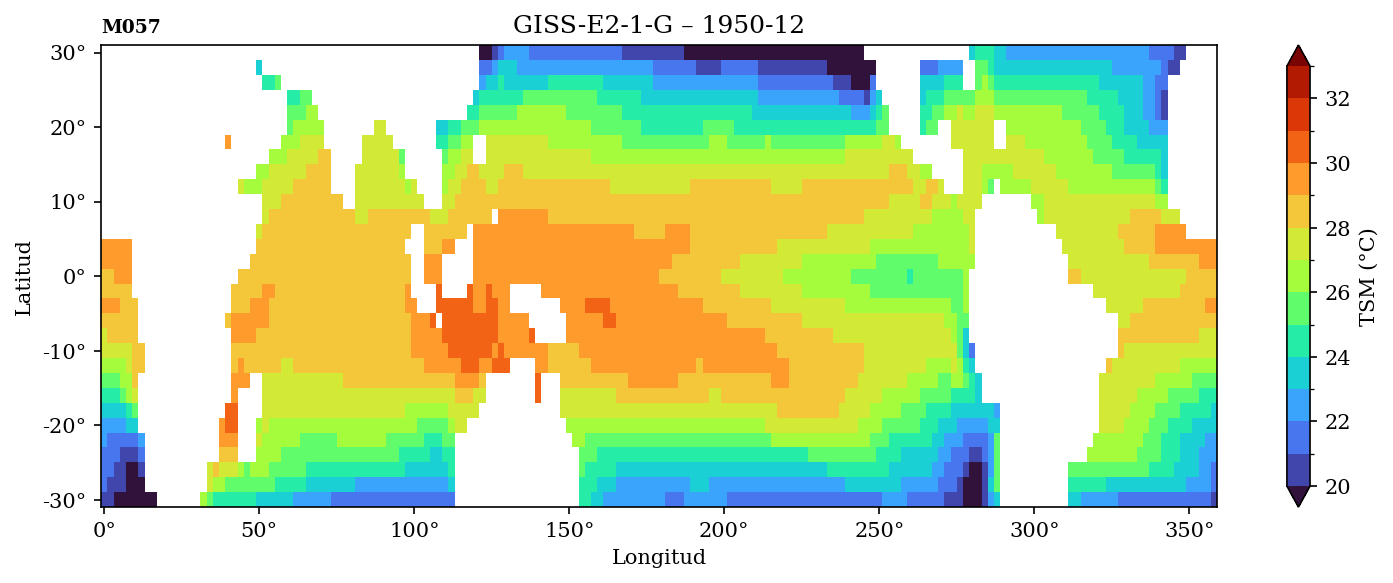
\includegraphics[width=\textwidth]{figuras/M057_sst_2d_GISS-E2-1-G.png}
\end{subfigure}
\caption[Campo de TSM de diciembre de 1950: ERSSTv5 y tres modelos de 250\,km.]{Temperatura superficial del mar de un mes de muestra (diciembre de 1950) en toda la ventana de descarga (0°--360°, 30°S--30°N), ya en la grilla, calendario, unidades y máscara océano-tierra comunes (Pasos~04--05). De arriba hacia abajo: ERSSTv5 y los modelos M001, M002 y M057 (Cuadro~\ref{tab:modelos}). Es una verificación visual de que todas las fuentes comparten grilla y máscara; al ser un mes aislado, no es una medida de desempeño.}
\label{fig:mapas2d}
\end{figure}

La Figura~\ref{fig:series} muestra la serie completa (\texttt{historical} y los tres escenarios SSP) de los mismos tres modelos en Niño~3.4, y la Figura~\ref{fig:boxplot} compara la distribución de la TSM histórica de ERSSTv5 y de los 40 modelos en ambas cajas.

\begin{figure}[htbp]
\centering
\begin{subfigure}[t]{\textwidth}
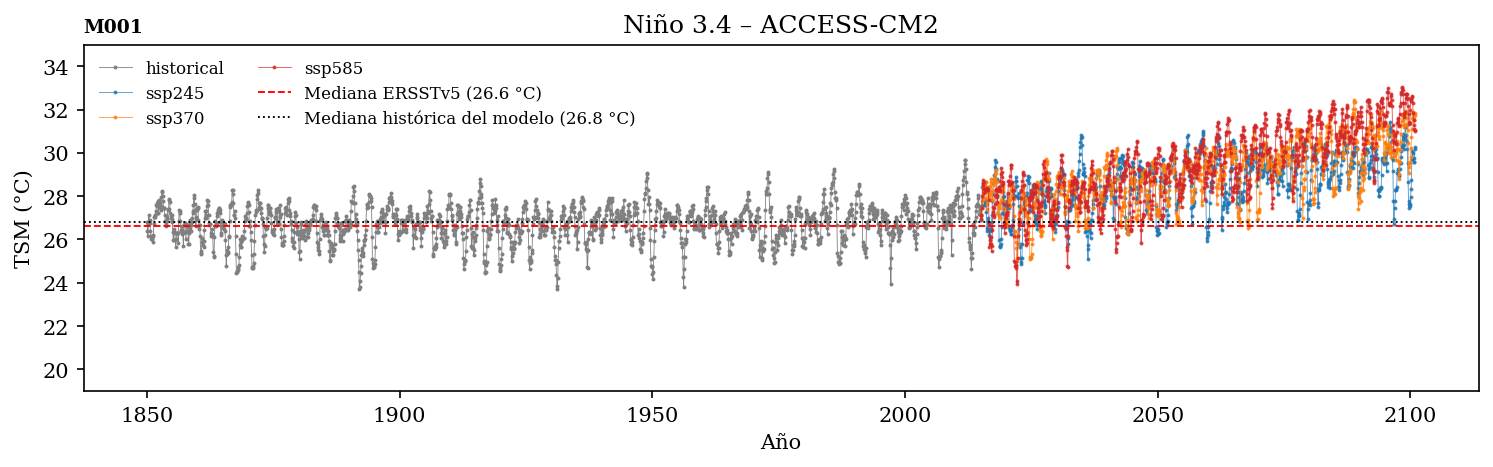
\includegraphics[width=\textwidth]{figuras/M001_serie_ACCESS-CM2_sst_Nino3.4.png}
\end{subfigure}
\begin{subfigure}[t]{\textwidth}
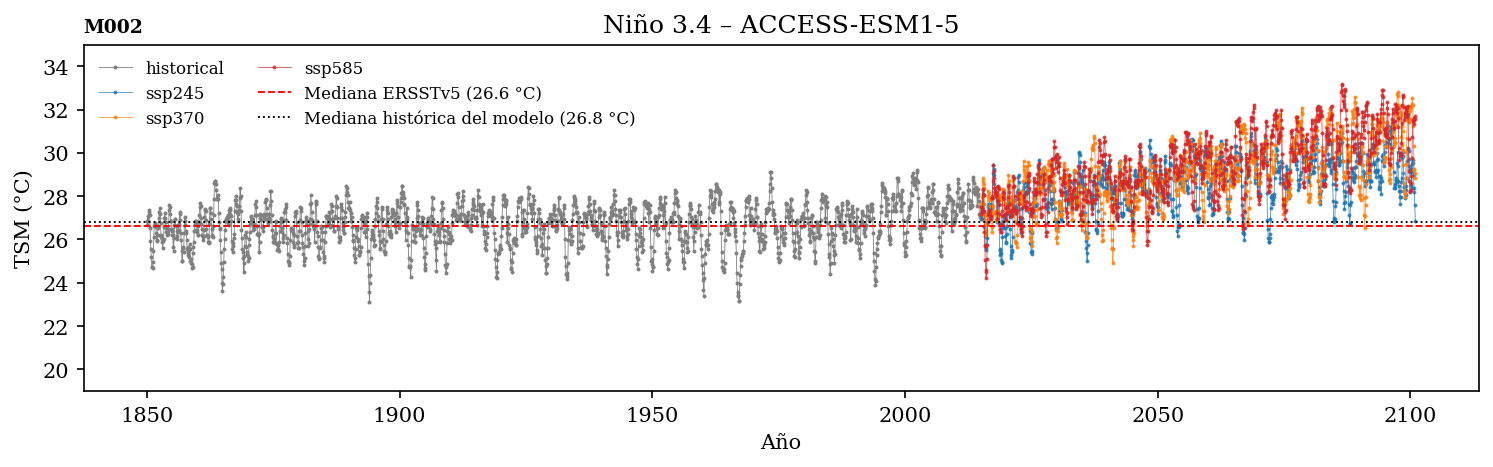
\includegraphics[width=\textwidth]{figuras/M002_serie_ACCESS-ESM1-5_sst_Nino3.4.png}
\end{subfigure}
\begin{subfigure}[t]{\textwidth}
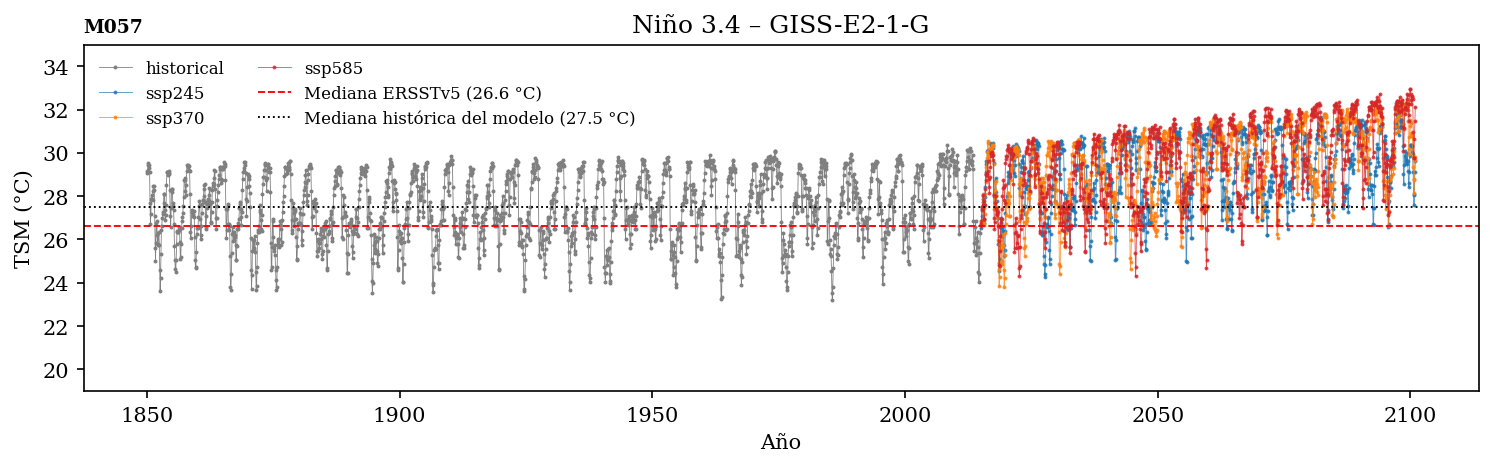
\includegraphics[width=\textwidth]{figuras/M057_serie_GISS-E2-1-G_sst_Nino3.4.png}
\end{subfigure}
\caption[Series de TSM en Niño~3.4 de tres modelos de 250\,km.]{TSM mensual promediada en Niño~3.4 (1850--2100): \texttt{historical} en gris y los tres escenarios SSP superpuestos, para los tres modelos de la Figura~\ref{fig:mapas2d}. Cada dato mensual se marca con un punto, sin interpolar huecos, de modo que un tramo sin puntos revelaría un hueco real de datos. Las líneas horizontales son la mediana de ERSSTv5 (roja, discontinua) y la mediana histórica del modelo (negra, punteada), ambas sobre el periodo común a las dos fuentes; su separación es el sesgo del modelo. El eje vertical es el mismo (19--35\,°C) en todos los paneles y en ambas cajas. Las series de Niño~1+2 se generan de la misma forma y se entregan junto con las demás figuras.}
\label{fig:series}
\end{figure}

\begin{figure}[htbp]
\centering
\begin{subfigure}[t]{\textwidth}
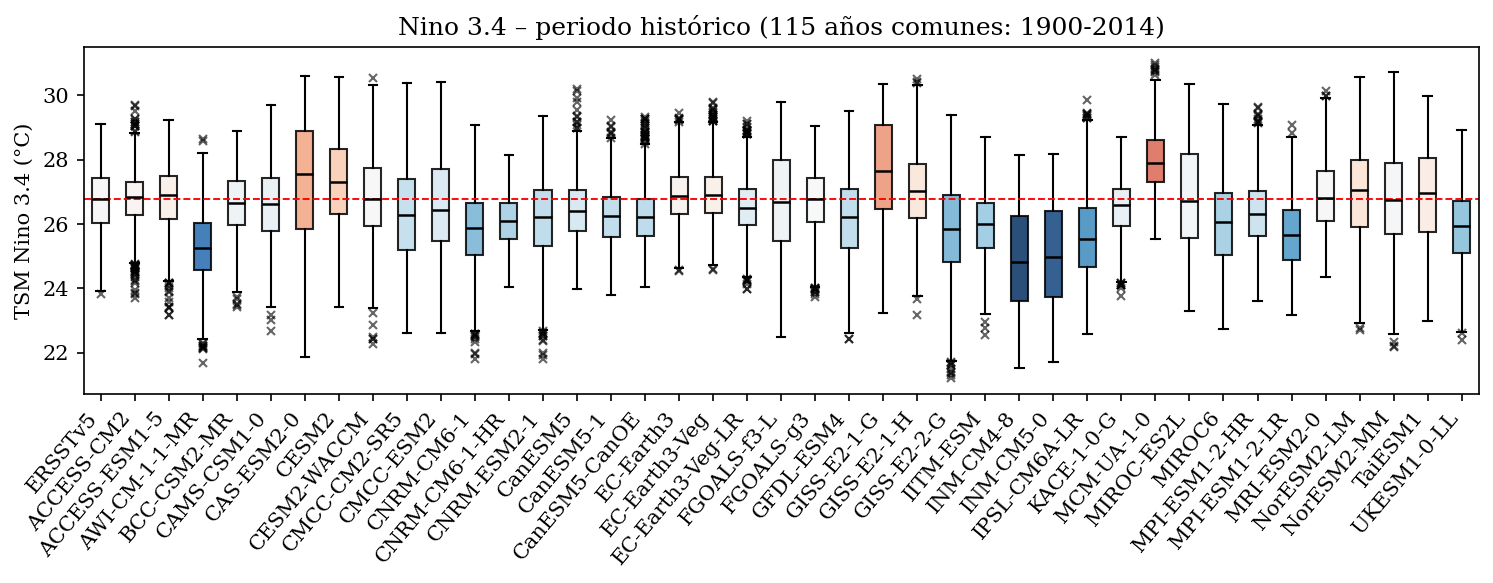
\includegraphics[width=\textwidth]{figuras/boxplot_Nino3.4.png}
\caption{Niño~3.4}
\end{subfigure}
\begin{subfigure}[t]{\textwidth}
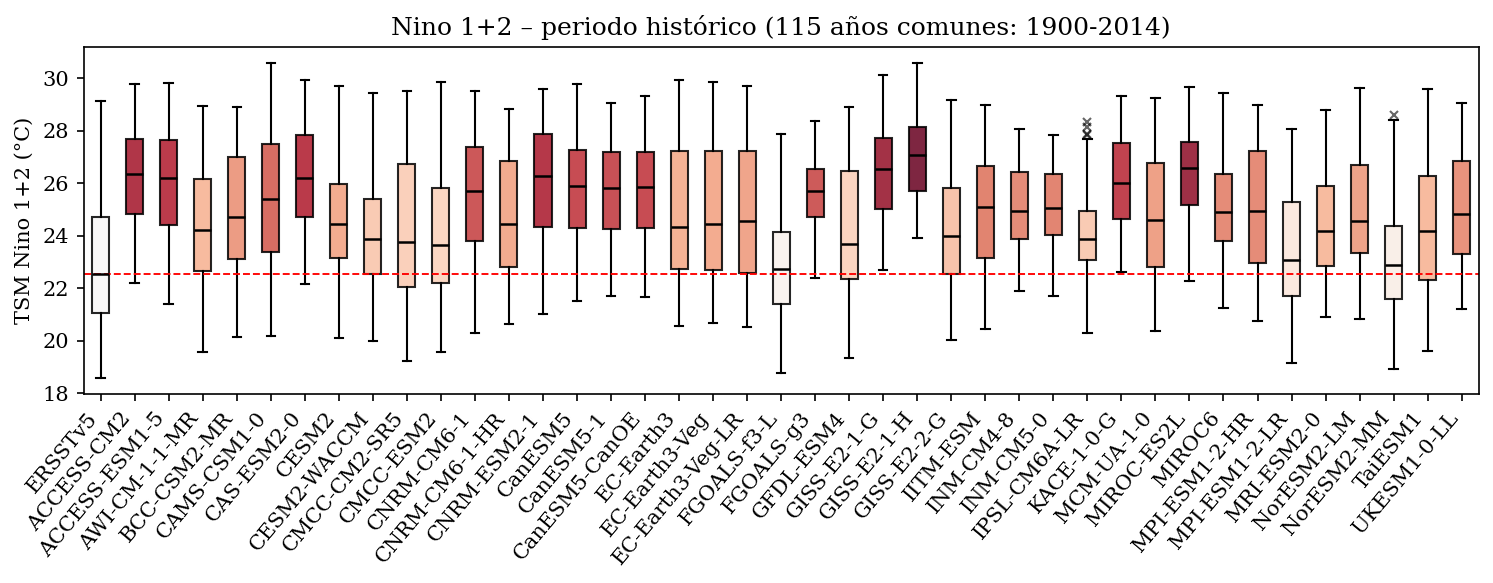
\includegraphics[width=\textwidth]{figuras/boxplot_Nino1+2.png}
\caption{Niño~1+2}
\end{subfigure}
\caption[Distribución de la TSM histórica en Niño~3.4 y Niño~1+2: ERSSTv5 frente a los 40 modelos.]{Distribución de la TSM mensual en cada caja para ERSSTv5 y los 40 modelos seleccionados, en el periodo común a todas las fuentes (1900--2014). Cada caja se colorea según la diferencia entre su mediana y la de ERSSTv5 (rojo, más cálido; azul, más frío); la línea roja discontinua marca la mediana observada.}
\label{fig:boxplot}
\end{figure}

Esta comparación preliminar ya anticipa un contraste entre cajas que el Entregable~2 deberá cuantificar. En Niño~3.4 la mediana de los modelos está cerca de la observada: 20 de los 40 modelos quedan a menos de 0{,}5\,°C de ERSSTv5 y el sesgo mediano es de $-0{,}24$\,°C. En Niño~1+2, 38 de los 40 modelos son más cálidos que la observación en más de 0{,}5\,°C, con un sesgo mediano de $+2{,}2$\,°C (rango de $+0{,}2$ a $+4{,}5$\,°C). Este sesgo cálido junto a la costa es coherente con lo señalado en la Sección~\ref{sec:similitudes} y con \citet{erickson2023}, quienes encuentran en la mayoría de los modelos CMIP6 un estado medio sesgado hacia condiciones de tipo El Niño, debido a sesgos cálidos de la TSM en el Pacífico tropical oriental. Refuerza la necesidad de reportar el sesgo de forma explícita y de calcular los índices como anomalías respecto de la climatología propia de cada modelo, de modo que el sesgo medio no se confunda con la variabilidad. La evaluación formal de desempeño (climatología, sesgos, diagrama de Taylor, índices ONI, RONI e ICEN) corresponde al Entregable~2.

\end{propuesto}

\bibliographystyle{plainnat}
\bibliography{../informe/references_rev}
\end{document}
